\documentclass{article}


% if you need to pass options to natbib, use, e.g.:
%     \PassOptionsToPackage{numbers, compress}{natbib}
% before loading neurips_2023


% ready for submission
% \usepackage{neurips_2023}
\usepackage[preprint]{neurips_2023}

% to compile a preprint version, e.g., for submission to arXiv, add add the
% [preprint] option:
%     \usepackage[preprint]{neurips_2023}


% to compile a camera-ready version, add the [final] option, e.g.:
%     \usepackage[final]{neurips_2023}


% to avoid loading the natbib package, add option nonatbib:
%    \usepackage[nonatbib]{neurips_2023}

\usepackage[utf8]{inputenc} % allow utf-8 input
\usepackage[T1]{fontenc}    % use 8-bit T1 fonts
\usepackage{hyperref}       % hyperlinks
\usepackage{url}            % simple URL typesetting
\usepackage{booktabs}       % professional-quality tables
\usepackage{amsfonts}       % blackboard math symbols
\usepackage{nicefrac}       % compact symbols for 1/2, etc.
\usepackage{microtype}      % microtypography
\usepackage{xcolor}         % colors
\usepackage{graphicx}

\title{Final Report: \\ Iterative Retrieval Augmented Generation through Subclaim Generation for Efficient Multi-Hop Fact Verification}


% The \author macro works with any number of authors. There are two commands
% used to separate the names and addresses of multiple authors: \And and \AND.
%
% Using \And between authors leaves it to LaTeX to determine where to break the
% lines. Using \AND forces a line break at that point. So, if LaTeX puts 3 of 4
% authors names on the first line, and the last on the second line, try using
% \AND instead of \And before the third author name.


\author{%
  Saeyoung Choi \\
  \texttt{saeyoung.choi@snu.ac.kr} \\
  \And
  Jinwha Jang \\
  \texttt{gdejin@snu.ac.kr}
  \And
  Yan GuangJing \\
  \texttt{mysnuguangjing@snu.ac.kr} \\
}

\begin{document}

\maketitle

\begin{abstract}
    Fact verification is an urgent problem which is even more crucial as the advent of generative language models. Retrieval augmented generation (RAG) approaches are combined with the large language models (LLM) to verify the factuality of claims with information retrieved from the knowledge base. However, the real-world sentences are often complex multi-hop claims, which are related to many different documents. To solve this problem, we propose the Iterative Retrieval Augmented Generation through Subclaim Generation model for efficient multi-hop fact verification. Instead of a single retrieval and generation, the proposed model conducts the iterative retrieval through generating subclaims. The model is evaluated with the fact verification datasets, using GPT-3.5-turbo as the base model. Although the proposed model shows higher performance than the simple retrieval model, it is inaccurate than the LLM-only model. In the further study, we should develop the method to process complicated relation between the different documents into the consistent context to verify the claim.
\end{abstract}

\section{Introduction}
As the cost of generating and delivering texts decreases, identifying misinformation and fact-checking becomes more important issues. Automatically generated misinformation is threatening to pollute the Internet. However, it is almost impossible to manually check the factuality of a massive number of texts generated by bots or language models. Hallucinations, plausible but incorrect text generation by language models, are also a difficult challenge to solve. Thus, the need for automated fact verification is urgent. With advances in natural language processing, attempts are being made to use various machine learning models for automatic fact verification \cite{chopra2017towards,zhong2019reasoning,nie2019combining}.\par
Recently, retrieval-augmented generation (RAG) \cite{lewis2020retrieval,izacard2020leveraging} is drawing attention for its potential in improving factuality of the language models \cite{shuster2021retrieval,ren2023investigating}. It can not only improve factuality but also provide explainability of the generated results, by utilizing both LLM's prior knowledge (parameters) and external knowledge (retrieved document). However, it is difficult to verify complex multi-hop claims. To verify multi-hop claims, the model should find several different relevant documents.\par
In this study, we propose a generative approach to enhance the model performance and efficiency, by utilizing generative capability of the language model for not only claim verification, but also retrieval. This approach includes (1) subclaim generation to verify the complex factuality within multi-hop claims, (2) document retrieval to obtain relevant evidence for each claim, and (3) claim verification based on the retrieved context. We will integrate them into our baseline model, and evaluate the performance of the integrated model.

\section{Related Work}

Iterative retrieval-generation synergy (ITRG) \cite{feng2023retrieval} is the iterative retrieval approach based on the LLM. Unlike the simple RAG model, it queries again with the generated results. Through this iterative procedure, the complex question related to the many different documents can be answered step by step. It can be considered as generating relevant documents by simultaneously exploiting parametric and non-parametric knowledge.

\begin{figure}[h]
  \centering
  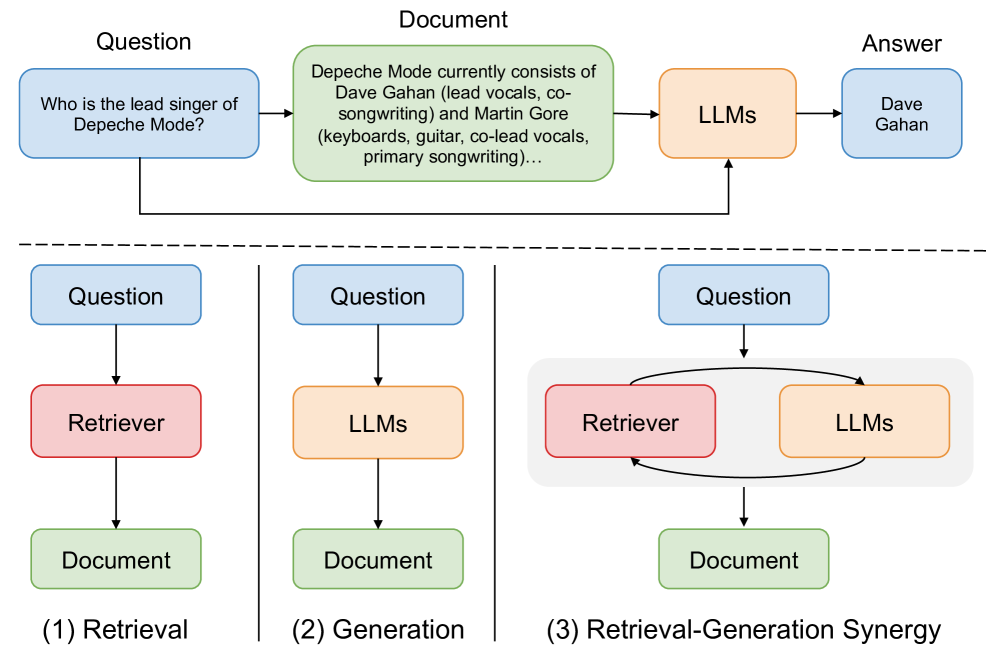
\includegraphics[width=0.6\linewidth]{Figure/itrg.png}
  \caption{The Architecture of the ITRG System}
\end{figure}

ITRG consists of two parts: generation augmented retrieval and retrieval augmented generation. In generation augmented retrieval, it concatenates the original question and the context, and uses it as query to retrieve the related documents. Then, in retrieval augmented generation, it reinforces the context with the generated results. By iterating this retrieval-generation-reinforcement process, the model can generate the context that integrates information from different documents.
\par

QACheck \cite{pan2023qacheck} adopts a question-guided multi-hop reasoning framework, significantly enhancing the clarity and effectiveness of fact-checking processes. Unlike traditional models that rely on linear evidence assessment, QACheck dissects complex claims into simpler components through a series of contextually relevant questions. This methodology not only increases the interpretability of the verification process but also aligns closely with human cognitive patterns in assessing veracity. \par

\begin{figure}[h]
  \centering
  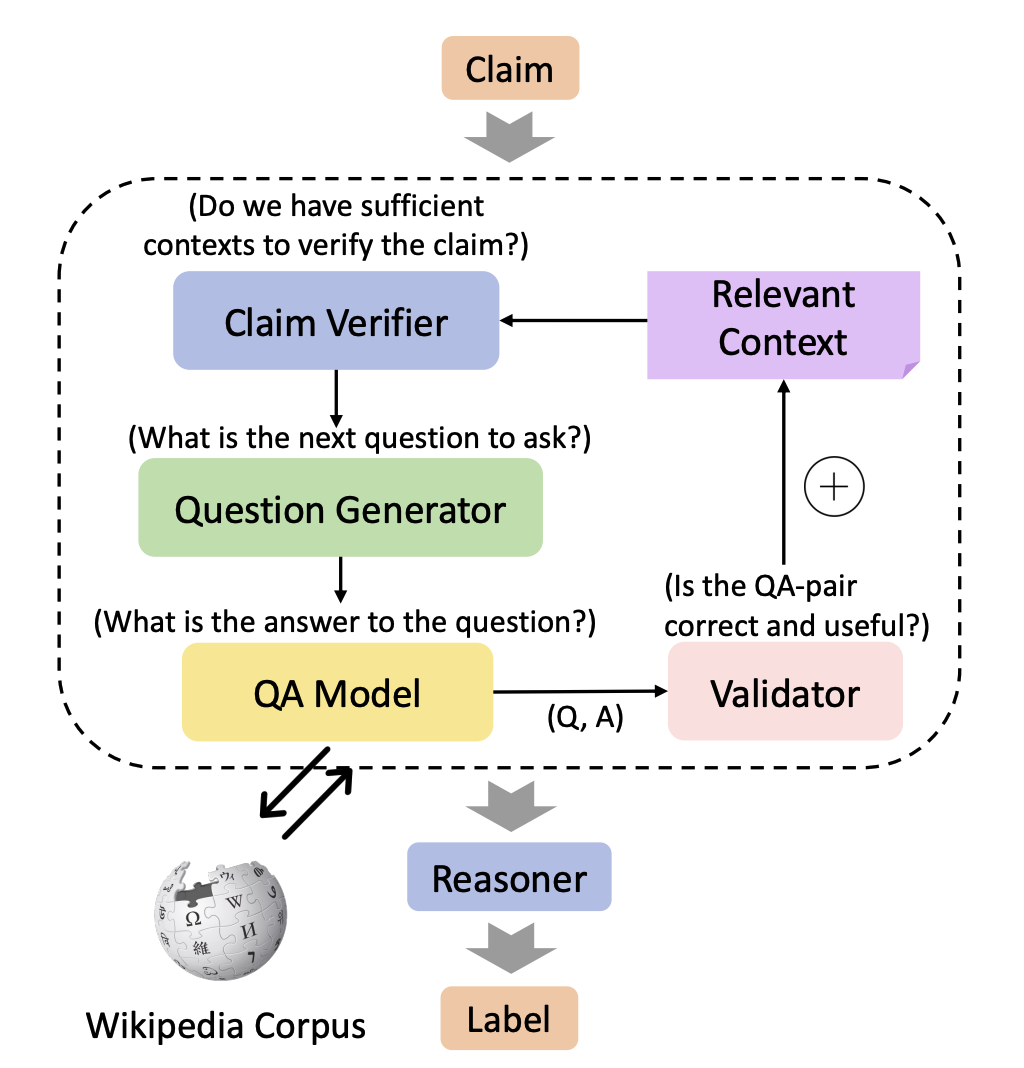
\includegraphics[width=0.4\linewidth]{Figure/Fig3.png}
  \caption{The Architecture of the QACheck System}
\end{figure}

The architecture of QACheck is a composite of five key modules: a claim verifier, a question generator, a question-answering module, a QA validator, and a reasoner. Each module plays a distinct yet interdependent role in the fact-checking pipeline. The claim verifier initially assesses the sufficiency of available context in substantiating a claim. Sequentially, the question generator and the QA module collaboratively work to explore and fill informational gaps. This synergy ensures a comprehensive examination of claims, thereby enhancing the accuracy of verification. 

\section{Model Description}

\subsection{Model Overview}
The fact verification task is to verify the factuality of the given claim. The proposed model utilizes the embedding model and the vector database for transforming, storing, and searching. LLM is used as the subclaim generator and the claim verifier. \autoref{bl} and \autoref{pp} shows the architecture of our baseline models and proposed model, respectively. \par

\begin{figure}[h]
  \centering
  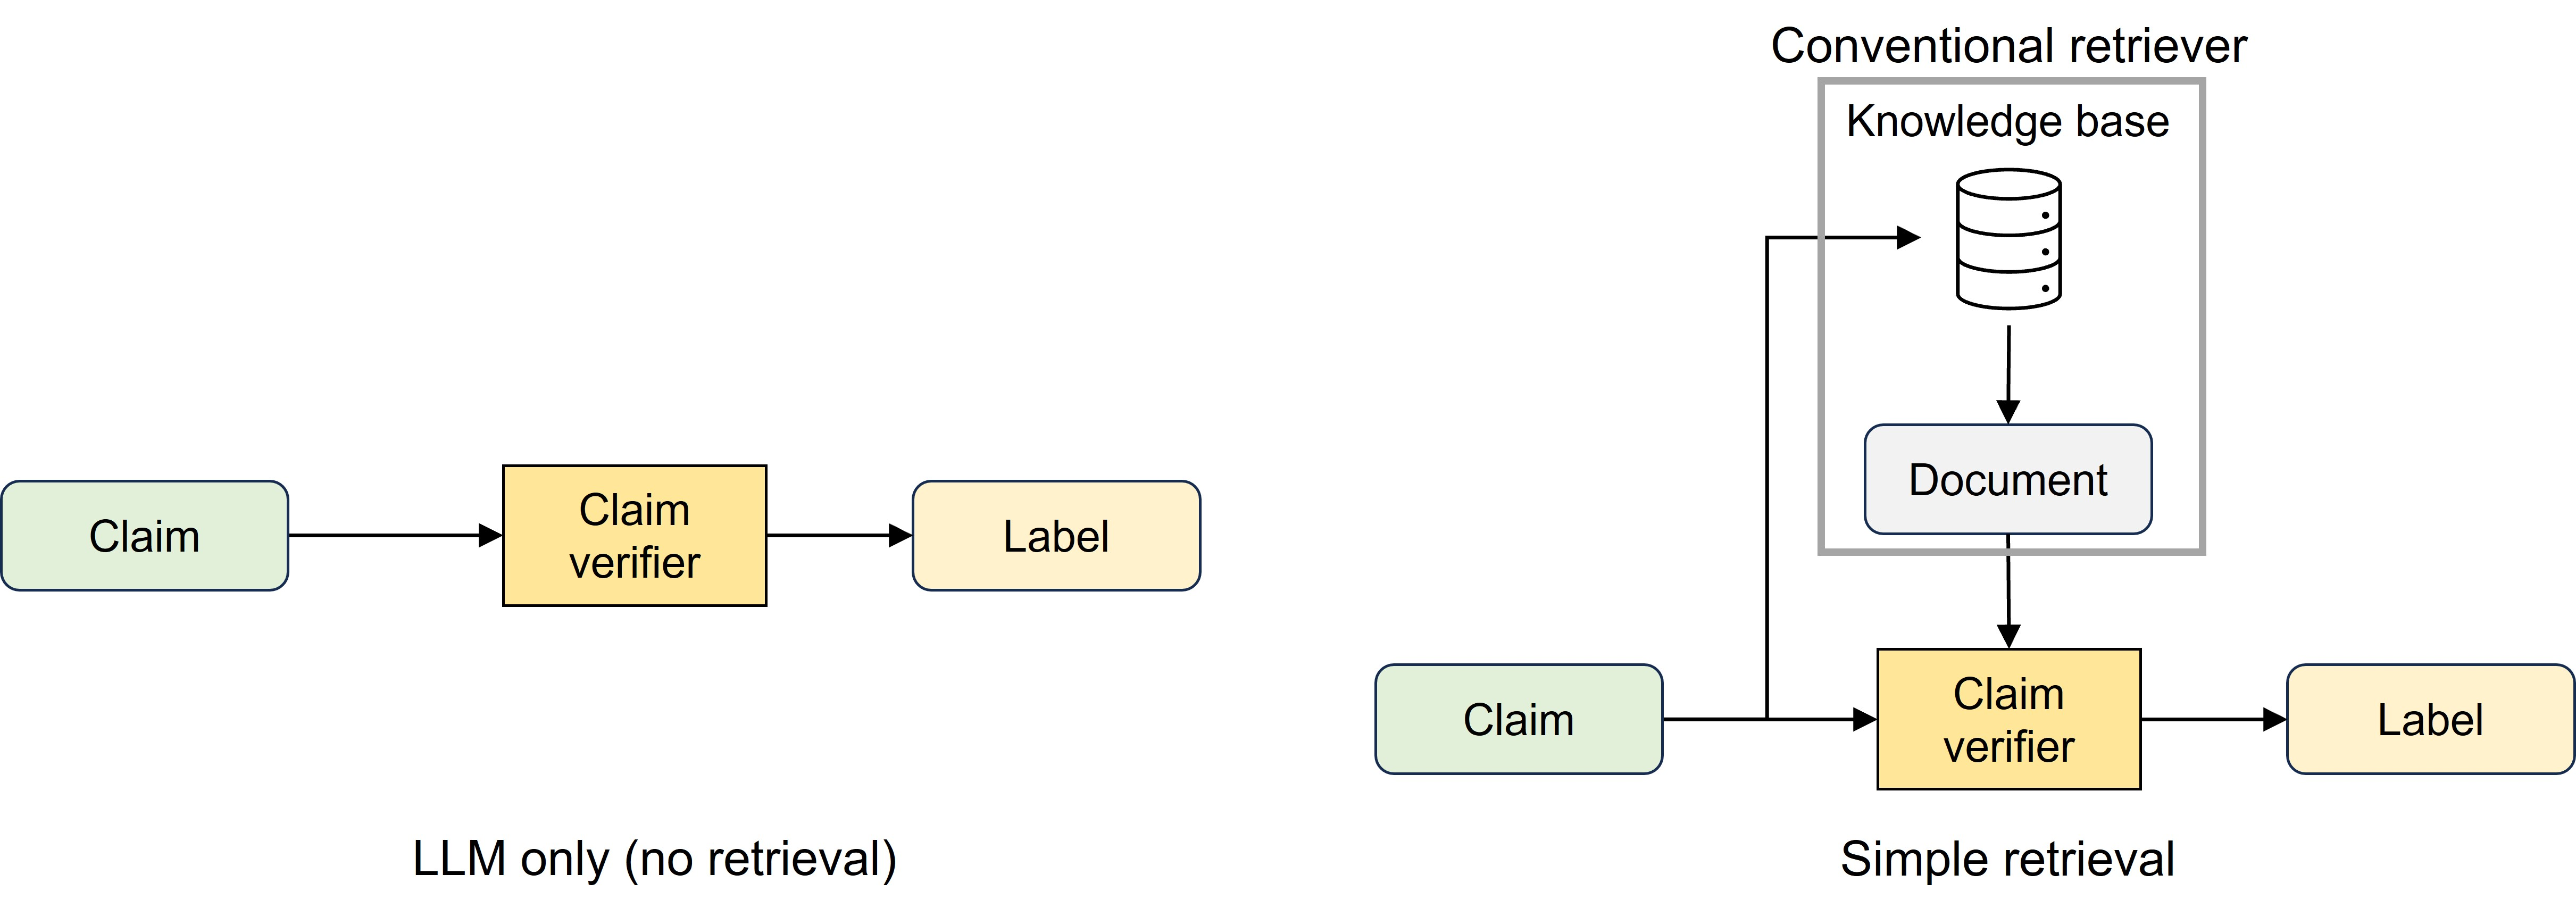
\includegraphics[width=0.95\linewidth]{Figure/fig1.jpg}
  \caption{\label{bl}Baseline Model Architecture}
\end{figure}
\begin{figure}[h]
  \centering
  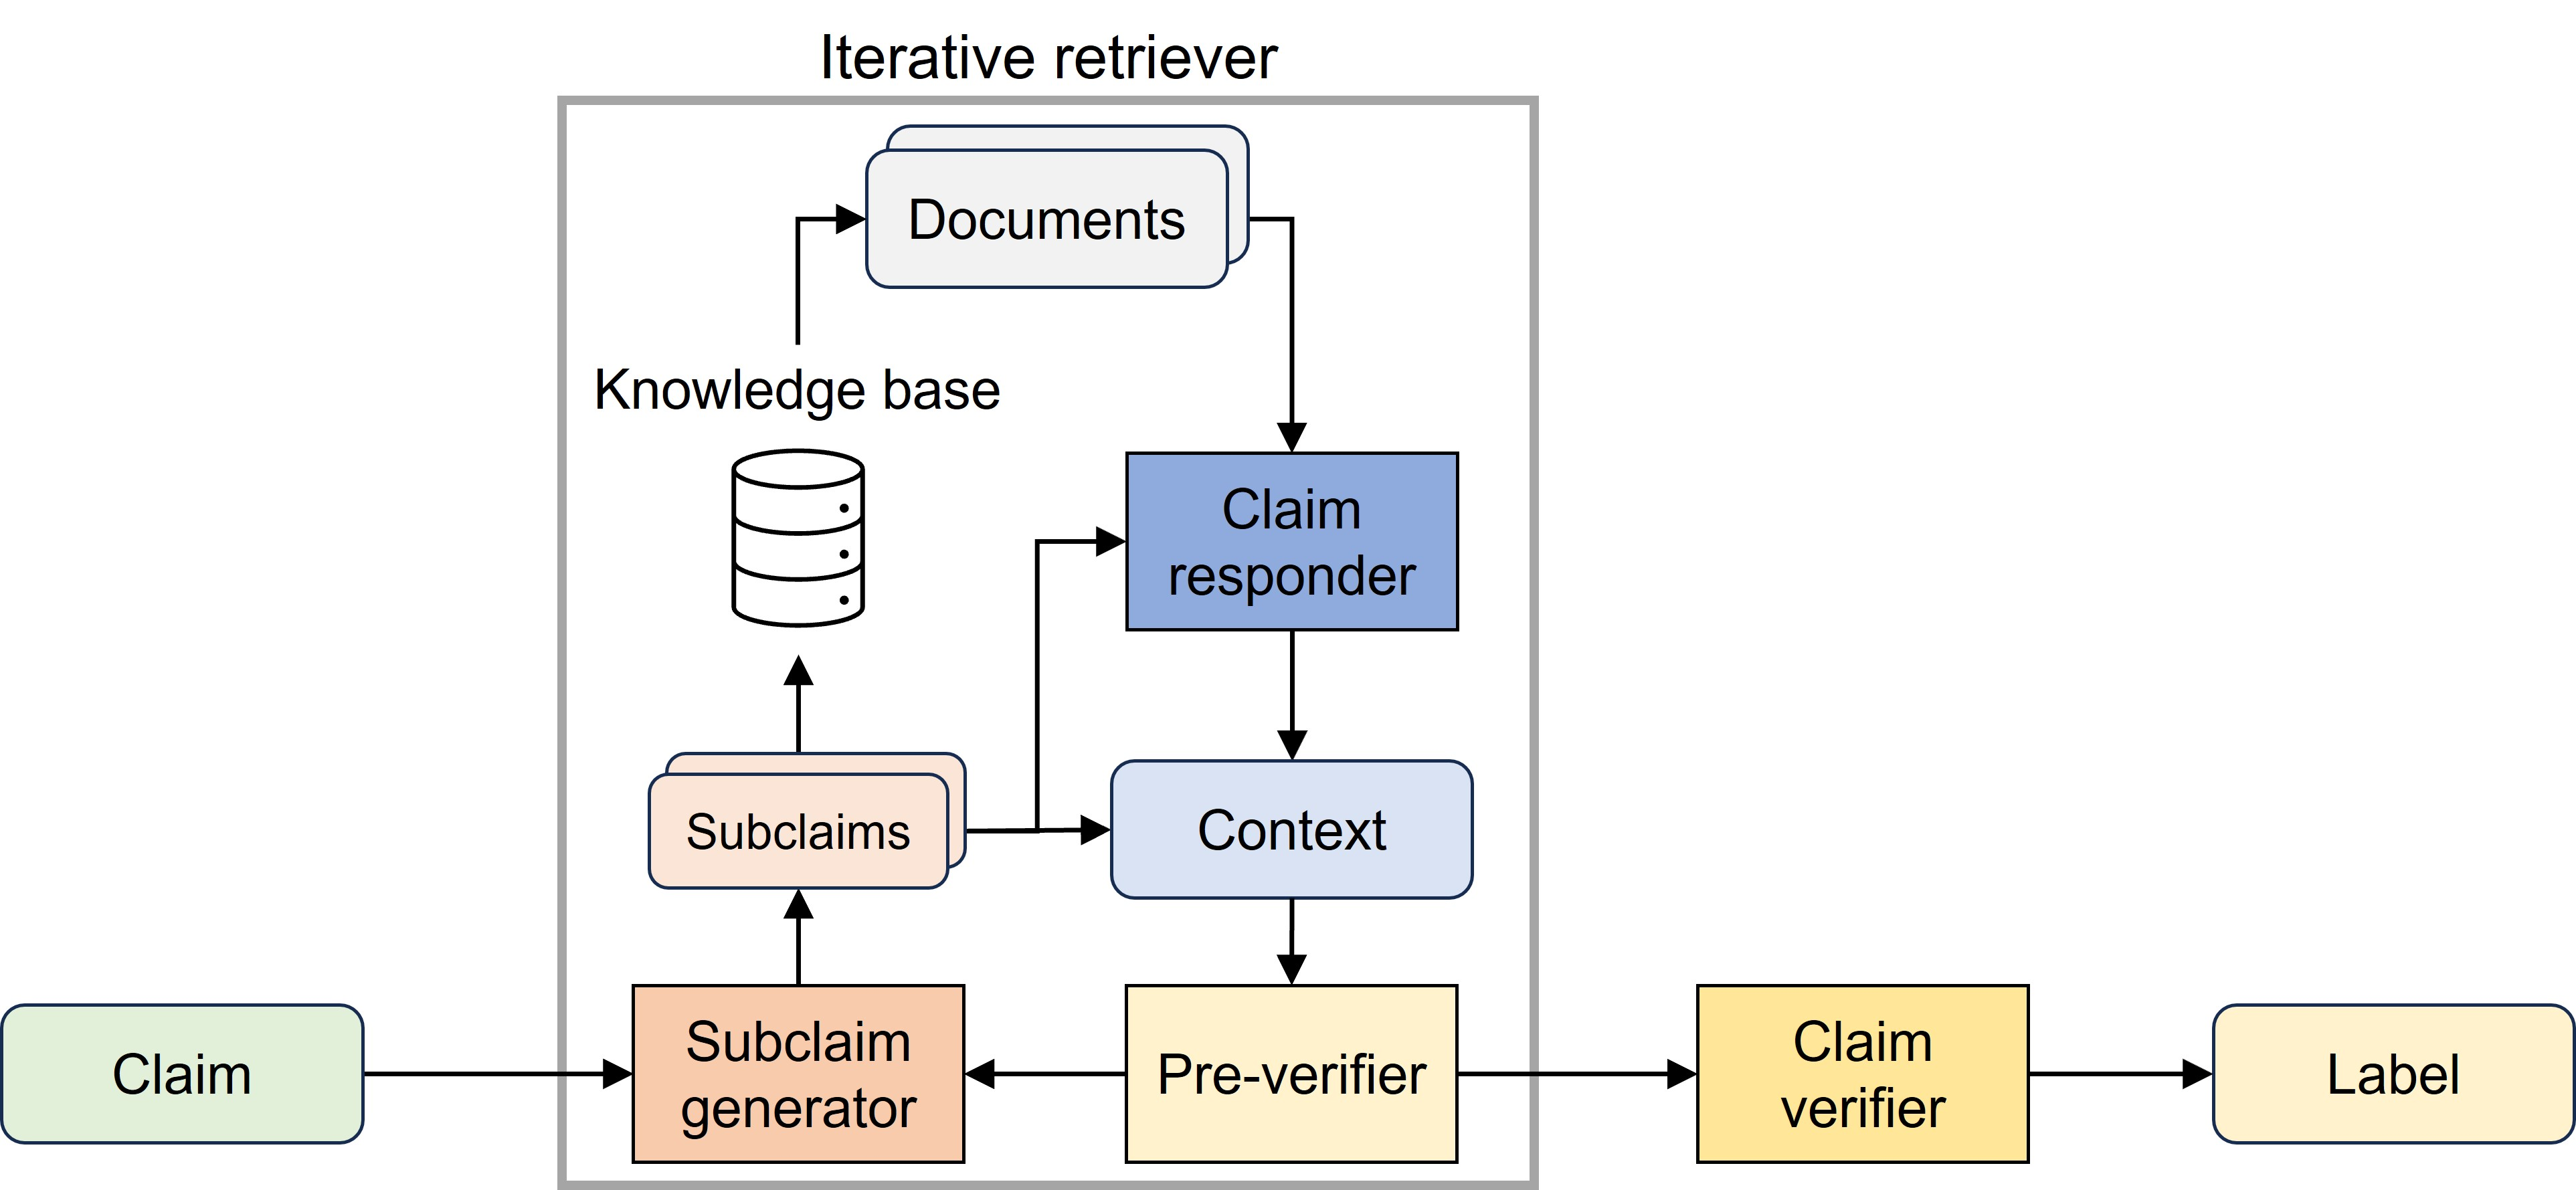
\includegraphics[width=0.75\linewidth]{Figure/fig2.jpg}
  \caption{\label{pp}Proposed Model Architecture}
\end{figure}

\subsection{Baseline model}\label{bs}
Two baseline models are presetned: LLM only (no retreival) and simple retrieval. In LLM only model, the LLM simply takes the given claim and verify it with its prior knowledge. The simple retrival model consists of retriever and claim verifier. The retriever first retrieves the documents that are similar to the given claim, by querying to the knowledge base. Claim and retrieved documents are put into the claim verifier, which then returns the factuality label (true or false).

\subsection{Proposed model}
While the simple retrieval model has conventional retriever and claim verifier, our proposed model consists of the following modules: (1) subclaim generator, (2) claim responder, (3) pre-verifier, and (4) claim verifier. \par
First, the subclaim generator breaks down complex claims into contextually relevant subclaims, through iterative procedure. At each 'round', the subclaim generator makes new subclaim based on the original claim and context.
Then, the claim responder answers to the generated subclaim through retrieval augment generation.
All generated subclaims and their responses are incorporated into the context.
Then, pre-verifier determines wheter the claim is verifiable with the given context. If not, it passes the context to the subclaim generator to generate new subclaim. 
If the context is sufficient, claim verifier makes the final verification.

\section{Experiment Setup}
Our model is constructed based on LlamaIndex \cite{LlamaIndex}, a framework for LLM-based application. 5,416,537 Wikipedia documents, which is the knowledge base from FEVER \cite{thorne2018fever} and HOVER \cite{jiang2020hover} dataset, are stored in vector database (pgvector on PostgresSQL), after transformed to embedding vectors with BAAI’s embedding model \cite{bge_embedding}. When a claim is given, it is transformed to a query embedding with the same sentence transformer. Then, the documents are retrieved from the knowledge base based on the similarity with the query embedding. The base model for subclaim generator, claim responder, pre-verifier, and claim verifier is GPT-3.5-turbo model \cite{gpt35}. 

\subsection{Dataset}
The proposed model is tested on claim samples from FEVER and HOVER datasets. They are open-domain fact verification dataset based on Wikipedia articles. While FEVER mostly has single-hop claims (related to a single document), HOVER has multi-hop claims (related to multiple documents). It should be noted that HOVER dataset has only two labels (Supported, Not supported) while FEVER dataset has three labels (Supports, Reputes, Not enough information) because of ambiguity between False and Not Verifiable in multi-hop claims. It is clearly shown that the conventional retrieval model fails to correctly verify the claims with multi-hop. Thus, in this study, we exclude the samples with Not enough information label in FEVER dataset for consistent comparison of the performance.

\subsection{Evaluation}
Overall fact verification performance of the model is evaluated through the F1 score. Retrieval performance is evaluated with the following retrieval score (RS).
$$\texttt{Retrieval score}=\frac{\sum_{i=1}^N s_i}{N}$$
where $N$ is the number of samples and $s_i$ is the score for the sample. In FEVER, if any of ‘evidence’ documents (documents when the sample claims are related) is retrieved successfully, $s_i=1$. In HOVER, which consists of multi-hop claims, the number of evidence documents retrieved is divided by the number of hops. For example, if only 1 evidence documents are successfully retrieved for 4-hop claim, $s_i=1/4$. \par
In previous literature, the reasoning (explanation) of the fact verification was evaluated manually by human experts \cite{zhang2023towards, wang2023explainable}. Some other literature \cite{kocmi2023large} provide the potential of LLM as a human-like evaluator. However, in this study, reasoning sentences are not evaluated.

\section{Result}
\subsection{Fact Verification Performance}
Fact verification performance, evaluated with F1 score, is shown in \autoref{tb1}. We compare three different models: LLM only (no retrieval), simple retrieval, and our proposed model. For 1-hop claims from FEVER dataset, proposed model achieve the highest F1 score. For multi-hop claims from HOVER dataset, the LLM only model has the best performance, while the proposed model shows higher performance than the simple retrieval model. \par
It can be interpreted that the LLM with the sufficient number of parameters have enough prior knowledge to verify the given claims. However, it still has the potential for improving the performance by the appropriate retrieval, as shown in 1-hop claims. \par
Low F1 score on the HOVER dataset can be explained with 'not enough information'. When the complex claim is given, LLM often reasons that the claim cannot be verified because of insufficient information (then answering as 'false'). The proportion of such cases (where reasoning includes 'cannot be verified', 'not possible', 'no evidence', or 'no mention') are shown in \autoref{tb2}. 

\begin{table}[h]
  \centering
  \begin{tabular}{c|c|ccc}
  \toprule
           & FEVER & \multicolumn{3}{c}{HOVER} \\ 
           & 1-hop & 2-hop   & 3-hop  & 4-hop  \\ \midrule
  LLM only (no retrieval) & 0.836  & 0.727  & 0.609   & 0.424   \\[0.5mm]
  Simple retrieval & 0.824  & 0.533 & 0.457  & 0.182   \\[0.5mm]
  Proposed model & 0.914  & 0.719    & 0.588   & 0.286   \\ \bottomrule
  
  \end{tabular}\\[5pt]
  \caption{\label{tb1}Fact verification performance (F1 score) of different models on FEVER and HOVER datasets}
\end{table}

\begin{table}[h]
  \centering
  \begin{tabular}{c|ccc}
  \toprule
           & \multicolumn{3}{c}{HOVER} \\ 
           & 2-hop   & 3-hop  & 4-hop  \\ \midrule
  Simple retrieval  & 0.694 & 0.786  & 0.953   \\[0.5mm]
  Proposed model  & 0.404   & 0.608   & 0.765   \\ \bottomrule
  
  \end{tabular}\\[5pt]
  \caption{\label{tb2}The ratio of 'not enough information' reasoning in HOVER dataset}
\end{table}

\subsection{Retrieval Performance}
The retrieval performance is evaluated to investigate the influence of hyperparameters. The retrieval score, which indicates how well 'evidence' documents are retrieved, is analyzed as shown in \autoref{k-rs} and 
\autoref{r-rs}. $k$ is hyperparameter that determines how many documents are retrieved in each retrieval (top-$k$). From \autoref{k-rs}, retrieval score increases gradually with increasing $k$. Regardless of hops, the number of documents should be decided carefully. Note that there may be trade-off due to an increase in the number of input context tokens. \autoref{r-rs} shows that the relationship between the maximum number of rounds and the retrieval score. It implies that the required number of rounds increases as the claim becomes complex. \par

\begin{figure}[h]
  \centering
  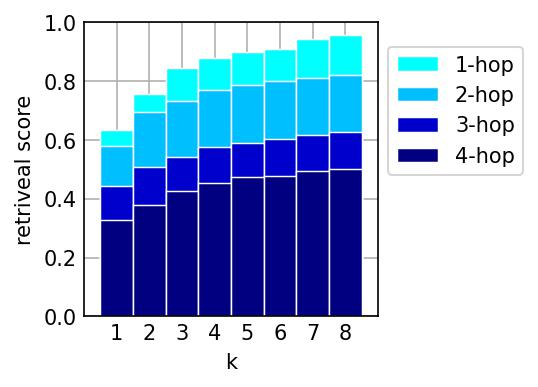
\includegraphics[width=0.6\linewidth]{Figure/k-rs.jpg}
  \caption{\label{k-rs}The retrieval score with the different number of retried documents (when number of rounds is 5)}
\end{figure}
\begin{figure}[h]
  \centering
  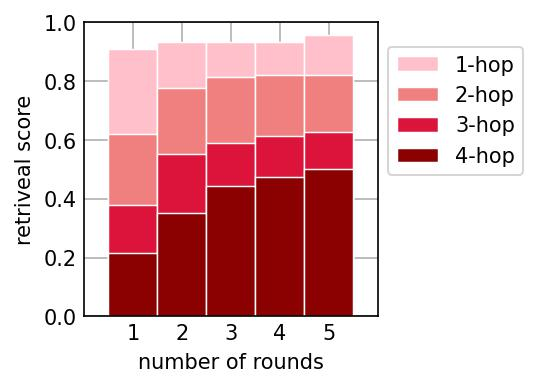
\includegraphics[width=0.6\linewidth]{Figure/rounds-rs.jpg}
  \caption{\label{r-rs}The retrieval score with the maximum number of rounds (when $k=8$)}
\end{figure}

\section{Conclusion}
In this study, we proposed the Iterative Retrieval Augmented Generation through Subclaim Generation model for complex fact verification problems. The fact verification performance and sensitivity to the hyperparameters were evaluated through the experiments. Although the proposed method was always more accurate than the simple retrieval model, it performed worse than LLM only model in multi-hop claims. Thus, we need to further investigate the followings:
\begin{itemize}
    \item How to generate better subclaims for complex claims
    \item How to process multiple retrieved documents into the consistent context
\end{itemize}
To generate better subclaims, structured methods like entity recognition for claim decomposition could be effective. Using the chain-of-thought reasoning as subclaim may be helpful, but it sometimes reinforce the hallucination through iterative process. \par

There are several limitations in this study. The results are dependent on the specific model (GPT-3.5-turbo). We should check whether the result (performance improvement) is rigid with different embedding models, database, and LLM. Trade-off between the LLM size (the number of parameters) and the performance must be investigated. Also, the proposed approach assumes that the documents retrieved from the knowledge base is always true. However, it is very costly to construct and maintain 'clean and truthful' knowledge base. Nowadays, search-based approach is becoming popular. Thus, the factuality of the retrieved documents (and logical consistency) should be also verified, using other documents and prior knowledge.


\bibliographystyle{unsrt}
\bibliography{References}

% \section*{Appendix: prompts}
% \subsection*{A.1.  Initial subclaim generation}
% Claim: \{claim\} \\
% To validate the above Claim, we need to ask a focused part question. What should be our first question? \\
% Question:

% \subsection*{A.2.  Follow-up subclaim generation}
% Below Known Information with Question \& Answer Contexts are collected so far: \\
% Context: \{context\} \\
% To further validate whether the claim is true or false, we need to ask a focused part question. What should be our next question? \\
% Question:

% \subsection*{A.3.  Retrieval augmented generation for subclaim}
% Context information is below. \\
% Context: \{context\} \\
% Question: \{subclaim\} \\
% Given the context information, answer the question.

% \subsection*{A.4.  Pre-verification}
% We are in the process of evaluating a claim through iterative questioning. Review the information collected so far: \\
% 1. Claim: \{claim\} \\
% 2. Q\&A Contexts: \{context\} \\
% Based on this information, then, clearly state if there is sufficient information to conclude whether "claim" is True or False: \\
% - 'More Information Needed' if the evidence is not conclusive and further questions are required. \\
% - 'Sufficient Information'  if the evidence clearly supports or refutes the claim. \\
% Label [More Information Needed/Sufficient Information]: 

% \subsection*{A.5.  Context processing}
% Question: \{subclaim\} \\
% Answer = \{answer\} \\
% Convert the above question-answer pair into a statement.

% \subsection*{A.6.  Fact verification}
% Context information is below. \\
% Context: \{context\} \\
% Claim: \{claim\} \\
% Given the context information, verify the claim. \\
% First, provide reasoning (within 100 words). Then, answer as [True, False] at the end. \\
% Reasoning: 

\end{document}